\chapter{Evaluation}    
  \section{Limitations}
    There are of course several limitations in Echo when compared to the original denotational semantics of FRP. Firstly, we are 
    unable to evaluate Behaviours at any time we choose.
    Although this does not limit much of the development of real-time, interactive applications there is some functionality
    lost. For instance it would be nice to be able to chart a Behaviour's value between certain bounds such as
    the trajectory of an object or a predetermined volume chart. This functionality can be provided with simple
    Time =$>$ T functions themselves but Behaviours could have provided a nice abstraction for these.
    
    The ability to transform Behaviours into different time frames is also lost due to the restriction on Behaviour
    evaluation. However, many of the use cases of this functionality can still be accomplished using the
    \emph{map} operation on Behaviours (such as slowing down or speeding up an animation Behaviour).
    
    The ability to use the \emph{predicate} operation is also removed. This function has not been included in any
    recent implementations (as discussed in chapter 3), most likely because of the reasons discussed in section~\ref{sec:time}. Some of the functionality offered by this function can be provided by the new \emph{filter} function for
    Events however:
    
\begin{verbatim}
val predicate = beh.sample(someEvent).filter(v => v == 5)
\end{verbatim}

    Although this doesn't offer the ability to find the exact point a continuous value meets some predicate we can
    use discrete sampling to provide similar, but far less accurate, functionality.
    
  \section{Efficiency}
    \label{sec:eff}
    As stated at the beginning of this report one of the goals of this project was to create an efficient implementation
    of FRP. More specifically, one that doesn't require an unbounded level of memory use due to storing Event occurrences.
    It is seen in section~\ref{sec:atomic} that this problem is avoided in Echo as Events only need to store their last
    occurrence. This not only means that Echo Events use a bounded amount of memory but it also means there is
    no overhead associated with throwing out old occurrences (the last occurrence is simply replaced with the new 
    one whenever the Event occurs).
    
    Also mentioned in section~\ref{sec:caching} Behaviour value caching is also used to prevent redundant reevaluation of 
    Behaviours
    and this further leads to a more optimised implementation of FRP. In a similar vein Echo does not redundantly recompute
    values for Behaviours lifted from constants. This is described in section~\ref{sec:lift}. This optimisation 
    allows for an efficient implementation of \emph{stepper} that
    doesn't revaluate its current phase on each evaluation (it simply returns the phase's value). This implementation is
    very similar to that suggested by Elliott's Reactive type (seen in chapter 3).
    
    There is a minor inefficiency due to the choice to make the \emph{occur} and \emph{eval} objects atomic
    with respect to all the FRP objects for an application. This means that even if two Behaviours or Events are in no way
    related they cannot be evaluated concurrently. It can be seen that in many applications the FRP objects will
    form disjoint groups of dependent Behaviours and Events. An optimisation to the framework could be to
    only lock access during \emph{occur} and \emph{eval} executions on a group by group basis rather than sharing
    a lock between all FRP object in an application. This would also allow unrelated Events to occur simultaneously.
  
  \section{Demo Applications}
    So as to gain experience with using Echo and also for the purposes of evaluation, demonstration
    applications were developed. 
    
    The first of these was a small music player application \ref{music-player}. The application
    can load in a `.wav' audio file and then play it back to the user. Pause and volume changing functionality
    is also available and the user is presented with a simple animation of the current volume level. One of the
    first points to cover is that an abstraction had to be built to enable the audio playback. This was in the form
    of a `Song' component. For this component playback is controlled by a Behaviour[Boolean] of whether the audio
    should be playing or not and the volume is dictated by a Behaviour[Int] that represents the current percentage
    volume. Once the abstraction was in place programming the FRP logic for the application using the 
    UI framework was very simple and, quite importantly, took very little time. It can be seen from
    the development of this application that abstractions over input and outputs would have to frequently be
    created to produce non-trivial FRP applications. However, any abstractions built would hopefully be
    reusable in nature due to FRPs high level approach to control. These findings also verify that it
    is important that Echo is as extendable as possible.
    
    Additional work was carried out on a small network anagram guessing game. This involved a server that provided
    an anagram and a client application that would present the anagram and allow the user to guess the original
    word. The user's answers would be reported to the server and the server would reply with whether
    the guess was correct or not. This application took advantage of the socket abstraction discussed in section~\ref{sec:io}
    and was actually very easy to develop with the Sender and Receiver types. Again, due to the functional and
    declarative nature of FRP the code for this application (both the server and the client) was very simple
    and intuitive to both create and read.
    
    Code excerpts from both demo applications can be seen in Appendix A and B. 
    
    \begin{figure}
      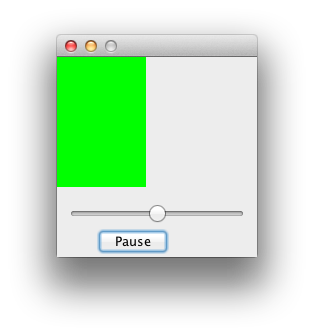
\includegraphics[width=\linewidth]{images/music-player.png}
      \caption{Music Player}
      \label{music_player}
    \end{figure}